\chapter{\label{ch:2-oxview}Nucleic acid structure design and analysis}
This chapter contains my results on how to design, simulate and analyse DNA and RNA nanostructures. It starts with an introductory description of earlier approaches to this problem and will then describe how my contributions to the oxView tool have improved the previous methods and enabled new results.

As I started this DPhil, I was tasked with the issue of converting origami designs created in caDNAno so that they can be correctly simulated in oxDNA.

I soon started collaborating with Hannah Fowler from the Doye group at Theoretical Chemistry. She was simulating a large collection of old DNA designs, so it was a good opportunity to convert and relax problematic structures, investigating why some structures are more problematic than others.

At this time, there was a python script included in the UTILS directory of the oxDNA repository, but it was difficult to use and it failed for many structures. At the end of 2018, the tacoxDNA webserver \cite{suma2019tacoxdna} was launched, updating the conversion script and making it more accessible. Still, since caDNAno structures are drawn on a lattice, the resulting oxDNA configurations often had unnaturally extended backbone bonds, requiring time-consuming relaxation.

During a secondment within the {\v{S}}ulc group at Arizona State University in 2019, I contributed to the development of a web-based oxDNA viewer called oxView\cite{poppleton2020design}. Among the main features I added to oxView was a cluster-level rigid-body dynamics option (detailed in Section \ref{sec:rigid-body_dynamics}) that in many cases speed up the relaxation with orders of magnitude compared to oxDNA relaxation alone. Since then I have been collaborating with the {\v{S}}ulc group to add more features and to make the tool more accessible as a visualiser and editor. For our second oxView publication I rewrote the main parts of the taxoxDNA codebase into typescript, resulting in the \emph{taxoxdna.js} library (\url{https://github.com/Akodiat/tacoxdna.js}) which oxView uses to import various common design formats automatically.

This section will present my own contributions to oxView, unless otherwise stated, but also I want to acknowledge the work done by Erik Poppleton and Michael Matthies; without them this tool would not exist. Michael was the original oxView developer and has done a great work in enabling live oxDNA relaxations through the \emph{ox-serve} webserver. Erik made oxView able to smoothly render and analyse systems with over a million nucleotides and has created a large set of handy analysis scripts.

\section{Importing designs}\label{sec:cadnanoConv}
There are a lot of different formats available for DNA origami design; some of the main design tools are covered in Section \ref{sec:design_tools}. This section will describe how to use oxView to import different designs.

\subsection{Basic import}
Thanks to the \emph{tacoxdna.js} library I created, the conversion is now straightforward for many designs. The formats listed below can all be imported by simply clicking the \emph{Import} button in oxview. Some additional formats still require the use of the external Tacoxdna webserver\cite{taco} however.
\subsubsection{Importing caDNAno files}
Select the caDNAno JSON file to import, making sure that \emph{caDNAno} is selected as file format. Next, select the correct lattice type; either \emph{Square} or \emph{Hexagonal}. Optionally, input a sequence to assign to the origami scaffold (which will otherwise be random).

\subsubsection{Importing rpoly files}
Rpoly files are the output from the BSCOR\cite{vHelix} tool (described in Section \ref{sec:bscor}) for converting polyhedral meshes into DNA origami.
Select the rpoly file to import, making sure that \emph{rpoly} is selected as file format. Optionally, input a sequence to assign to the origami scaffold (which will otherwise be random).

\subsubsection{Importing Tiamat files}
Select the tiamat \emph{.dnajson} file to import, making sure that \emph{tiamat} is selected as file format. Binary \emph{.dna} Tiamat files need to be reopened in Tiamat and saved to the text-based \emph{.dnajson}. Select Tiamat version (1 or 2), then select nucleic acit type (DNA or RNA).

By default, nucleotides without assigned base types will be given a random type. However, it is also possible to select a fixed default base.

\subsubsection{Importing PDB files}
While I did create include the DNA PDB to oxDNA converter from Tacoxdna in \emph{tacoxdna.js}, a more versatile PDB import was created by Jonah Procyk to support his ANM-oxDNA model \cite{procyk2021coarse}. Simply drag and drop (or load) a PDB file into an oxView window and the DNA, RNA and/or protein it contains will be automatically converted and loaded.

%The simplest method is now to use the recently published tacoxDNA web service\cite{suma2019tacoxdna} (whose conversion script is more or less the same as in the oxDNA repository). However, the script can still fail to parse some designs, so a future implementation that uses the native caDNAno library for parsing would be preferable.

\subsection{Multi-component designs}
Designs spread across multiple files (or even multiple design tools) can be easily combined in oxView by simply importing them all and using the editing tools to arrange and connect them properly.

\subsection{Far-from-physical caDNAno designs}
Some structures, while converted without failure to the oxDNA format, will have a very far-from-physical configuration due to the way they are drawn in caDNAno. As mentioned above, since it is only possible to draw all helices parallel to each other, on a lattice, backbone bonds may be very elongated, creating high energies and/or topological problems.

The oxDNA software already includes relaxation procedures for such structures, bringing them together in a slow and controlled manner using a specified maximum backbone force. However, for large structures, this can take a very long time, even while using GPU simulation.

In such cases, another software I have investigated, called mrdna (Multi-resolution DNA nanotechnology), proves very useful\cite{maffeo2018}. It is a python package using ARBD (Atomic Resolution Brownian Dynamics), both being developed by Chris Maffeo, to simulate double- and single-stranded DNA structures at multiple levels of coarse-graining. Since these simulations are more coarse-grained than oxDNA, they run significantly faster. Furthermore, after I have been in contact with Chris, mrdna can now also be configured to output and simulate oxDNA configurations as the final simulation step. Because of this, mrdna can also be useful for converting simple structures, if tacoxDNA fails to parse the caDNAno file.

\section{Rigid-body manipulation and dynamics}
\label{sec:rigid-body_dynamics}
Rapid relaxation of converted cadnano designs

Rigid-body manipulation \cite{huang2019uncertainty}. The translation and rotation tools in oxView allow users to select and rearrange blocks of nucleotides as rigid bodies. 

Dynamics \cite{baraff1997introduction}

Manually, on import or through DBSCAN algorithm \cite{ester1996density}.

Clusters held together with spring forces at each shared backbone bond, with a magnitude of 
$$ f_{\rm spr} = c_{spr}(l - l_r),$$
where \(c_{spr}\) is a spring constant, \(l\) is the current bond length and \(l_r\) is the relaxed bond length. To avoid overlaps, a simple linear repulsive force, of magnitude
$$ f_{\rm rep} = max\left(c_{rep}\left(1-\frac{d}{r_a+r_b}\right),0\right)$$ is added between the centre of each group, where \(c_{rep}\) is a repulsion constant, \(d\) is the distance between the two centres of mass, and \(r_a+r_b\) is the sum of the group radii (the greatest distance they can be while still overlapping).

\begin{figure}
\centering\includegraphics[width=\textwidth]{figures/icosahedron.png} 
\caption{Rigid-body dynamics of clusters. Snapshots from the automatic rigid-body relaxation of an icosahedron, starting with the configuration converted from caDNAno \textbf{a)}, through the intermediate \textbf{b)} where the dynamics are applied, and \textbf{c)} the final resulting relaxed state.}
\label{fig:rigidBody}\end{figure}

\section{Editing designs}

\begin{figure}
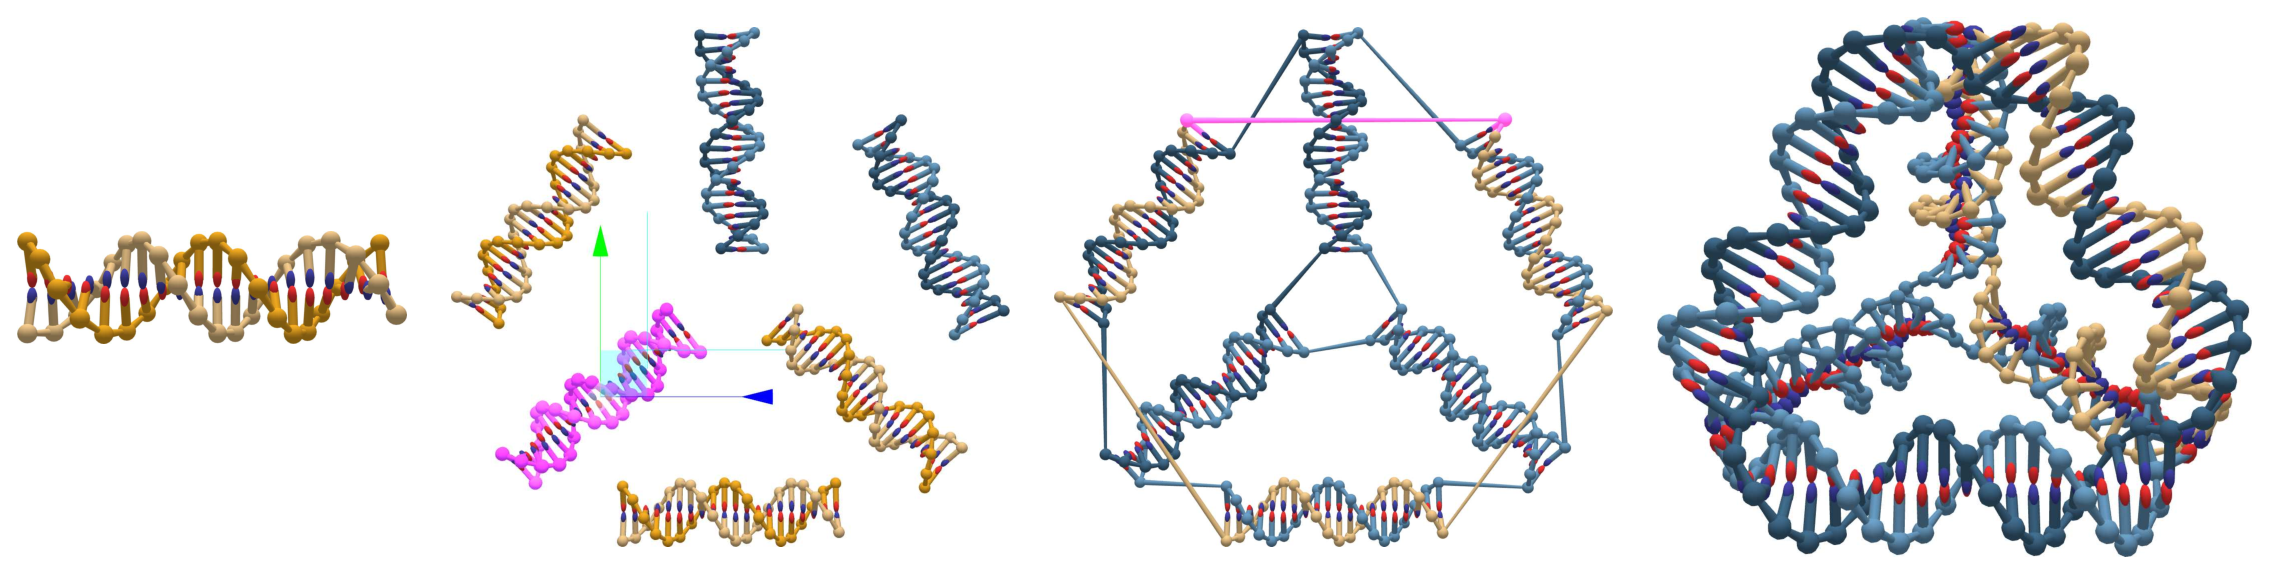
\includegraphics[width=\textwidth]{figures/tetra.eps} 
\caption{Designing the DNA tetrahedron from \cite{goodman2005rapid} using the oxView editing tools. a) The initial helix created. b) Duplicated helices being translated into place. c) Strands ligated together. d) The resulting 3D tetrahedron shape, as seen after applying rigid-body dynamics.}
\label{fig:design}
\end{figure}

%ligate, nick, do/undo, extend and create strands

\newcommand{\toolHeight}{1.5em}


\begin{table}[h!]
\centering

\begin{tabularx}{\textwidth} { >{\centering\arraybackslash}m{3em} | X }
 \hline
 Tool & Description \\ [0.5ex] 
 \hline
 \hline
\includesvg[height=\toolHeight]{figures/tools/create} & \textbf{Create} a new strand from a given sequence. Select \textit{duplex mode} to instead create a helix. \\ \hline
\includesvg[height=\toolHeight]{figures/tools/copy} & \textbf{Copy} the selected elements (Ctrl+C). \\ \hline
\includesvg[height=\toolHeight]{figures/tools/cut} & \textbf{Cut} the selected elements (Ctrl+X). \\ \hline
\includesvg[height=\toolHeight]{figures/tools/paste} & \textbf{Paste} elements from clipboard (Ctrl+V to paste in original position, or Ctrl+Shift+V to paste in front of camera). \\ \hline
\includesvg[height=\toolHeight]{figures/tools/delete} & \textbf{Delete} all currently selected elements. (delete) \\ \hline
\includesvg[height=\toolHeight]{figures/tools/ligate} & \textbf{Ligate} two strands by selecting the 3' and 5' endpoint elements to connect (L) \\ \hline
\includesvg[height=\toolHeight]{figures/tools/nick} & \textbf{Nick} a strand at the selected element (N) \\ \hline
\includesvg[height=\toolHeight]{figures/tools/extend} & \textbf{Extend} strand from the selected element with the given sequence. Select \textit{duplex mode }to also extend the complementary strand. \\ \hline
\includesvg[height=\toolHeight]{figures/tools/insert} & \textbf{Insert} (add) elements within a strand after the selected element \\ \hline
\includesvg[height=\toolHeight]{figures/tools/skip} & \textbf{Skip} (remove)  selected elements within a strand. \\ \hline
\includesvg[height=\toolHeight]{figures/tools/rotate} & \textbf{Rotate} selected elements around their center of mass (R). \\ \hline
\includesvg[height=\toolHeight]{figures/tools/translate} & \textbf{Translate} currently selected elements (T). \\ \hline
\includesvg[height=\toolHeight]{figures/tools/moveto} & \textbf{Move to}. Move other selected elements to the position of the most recently selected element. \\ \hline
\includesvg[height=\toolHeight]{figures/tools/connect3s} & \textbf{Connect 3' duplex}. Connects the 3' ends of two selected staple strands with a duplex, generated from the sequence input. \\ \hline
\includesvg[height=\toolHeight]{figures/tools/connect5s} & \textbf{Connect 5' duplex}. Connects the 5' ends of two selected staple strands with a duplex, generated from the sequence input. \\ \hline
\includesvg[height=\toolHeight]{figures/tools/set} & \textbf{Set} the sequence of currently selected elements. Select duplex mode to also set the complementary sequence on paired elements. \\ \hline
\includesvg[height=\toolHeight]{figures/tools/get} & \textbf{Get}. Assigns the sequence of selected bases to the sequence input.  \\ \hline
\includesvg[height=\toolHeight]{figures/tools/rc} & \textbf{Reverse complement}. Generates the reverse complement of a provided sequence. \\ \hline
\includesvg[height=\toolHeight]{figures/tools/search} & \textbf{Search}. Highlights the position the provided sequence in each strand, if present. \\ \hline
\end{tabularx}

\caption{Editing tools available in oxView}
\label{table:edit_tools}
\end{table}



\begin{figure}
\centering\includegraphics[width=\textwidth]{figures/oxdna_sims.eps} 
\caption{Relaxation results for various DNA designs. Each row depicts a new design, with the left-hand side showing the structure as it was drawn in caDNAno (and parsed by mrdna), while the right-hand side is the relaxed structure in oxDNA. Intermediate images are edits done in mrdna. While the switch design\cite{gerling2015dynamic} in \textbf{a)} 
and the small DNA origami box\cite{zadegan2012smallbox} in \textbf{b)} relaxed without any required editing, the tensegrity kite structure \cite{liedl2010_kite} in \textbf{c)} and the Möbius strip\cite{han2010moebius} in \textbf{d)} benefited greatly from moving selected helices to a position off the lattice before starting the simulation.}
\label{fig:oxDNA_sims}\end{figure}

\section{Example conversions}
A selection of the DNA designs I have relaxed are shown in Figure \ref{fig:oxDNA_sims}. The first two examples, adopted from \cite{gerling2015dynamic} and \cite{zadegan2012smallbox} and illustrated in Figure \ref{fig:oxDNA_sims}.a and \ref{fig:oxDNA_sims}.b, are both quite straightforward to relax in oxDNA, although the relaxation is much faster using mrdna.

The tensegrity kite structure, adopted from \cite{liedl2010_kite} is harder to relax since, as seen in the first image in Figure \ref{fig:oxDNA_sims}.c, the two helix bundles are drawn parallel to each other in caDNAno. Given enough time to relax, they should still become orthogonal, but a much more efficient way is to write a mrdna script to rotate one helix bundle so that it is orthogonal from the start, as seen in the middle image of \ref{fig:oxDNA_sims}.c. The remaining overstretched bonds are then quickly relaxed using mrdna.

Finally, the Möbius strip, adopted from \cite{han2010moebius}, is particularly tricky to relax, since the caDNAno design have all helices drawn in the same plane, with bonds from each end stretching through the whole structure and intersecting at a single point, as can be seen in the first image of Figure \ref{fig:oxDNA_sims}.d. With some help from Chris Maffeo, however, I was able to use a mrdna script to edit the structure into a configuration much easier to relax, as seen in the second image of Figure \ref{fig:oxDNA_sims}.d. Since the caDNAno design does not make it clear if the Möbius strip should be left-handed or right-handed, this is also decided in the script; changing the rotational direction will produce a mirrored version of the structure, as seen in the third image of Figure \ref{fig:oxDNA_sims}.d.

\section{Visualization options}
Centring with periodic boundary conditions

Change component sizes, change colours, fog., virtual reality, glTF in blender.

\begin{figure}
\centering\includegraphics[width=\textwidth]{figures/oxview.png} 
\caption{Screenshot of the online oxView tool, exporting a video of a slider on a rail from a simulated trajectory.}
\label{fig:oxview}\end{figure}

\section{Exporting designs}
Video, image, 3D files, sequence files, oxDNA simulation files.


\section{Converting RNA origami designs}
During my secondment at the Andersen lab in Aarhus, I worked with converting RNA structures designed using their ASCII-based blueprint format into oxRNA simulation files. Examples of converted structures are shown in Figure \ref{fig:oxRNA_sims}. The Andersen lab already has scripts, soon to be published, for parsing their blueprint files and building the corresponding PDB structures (the first two columns of Figure \ref{fig:oxRNA_sims}). However, the resulting PDB files are not relaxed and would take a long time to relax using all-atom simulation. As such, I modified the tacoxDNA \cite{suma2019tacoxdna} PDB parser to enable PDB-to-oxRNA conversion. I have contacted Lorenzo to let him know about these additions and hopefully, they will be included in a future version of tacoxDNA. One issue I noticed with the conversion was that the asterisk (*) and prime (') characters were used interchangeably in the RNA motif library to name atoms of the sugar group, causing problems with the tacoxDNA script, which only recognises the prime. This has already been fixed in tacoxDNA. The third column of Figure \ref{fig:oxRNA_sims} shows the structures relaxed and simulated in oxRNA, some significantly different from the previously available PDB models in the second column.

% "The asterisk (*) is used in place of the prime character (') for naming atoms of the sugar group" - https://cdn.rcsb.org/wwpdb/docs/documentation/file-format/PDB_format_1996.pdf

\begin{figure}
\begin{center}
\makebox[\textwidth][c]{a)  
  \centering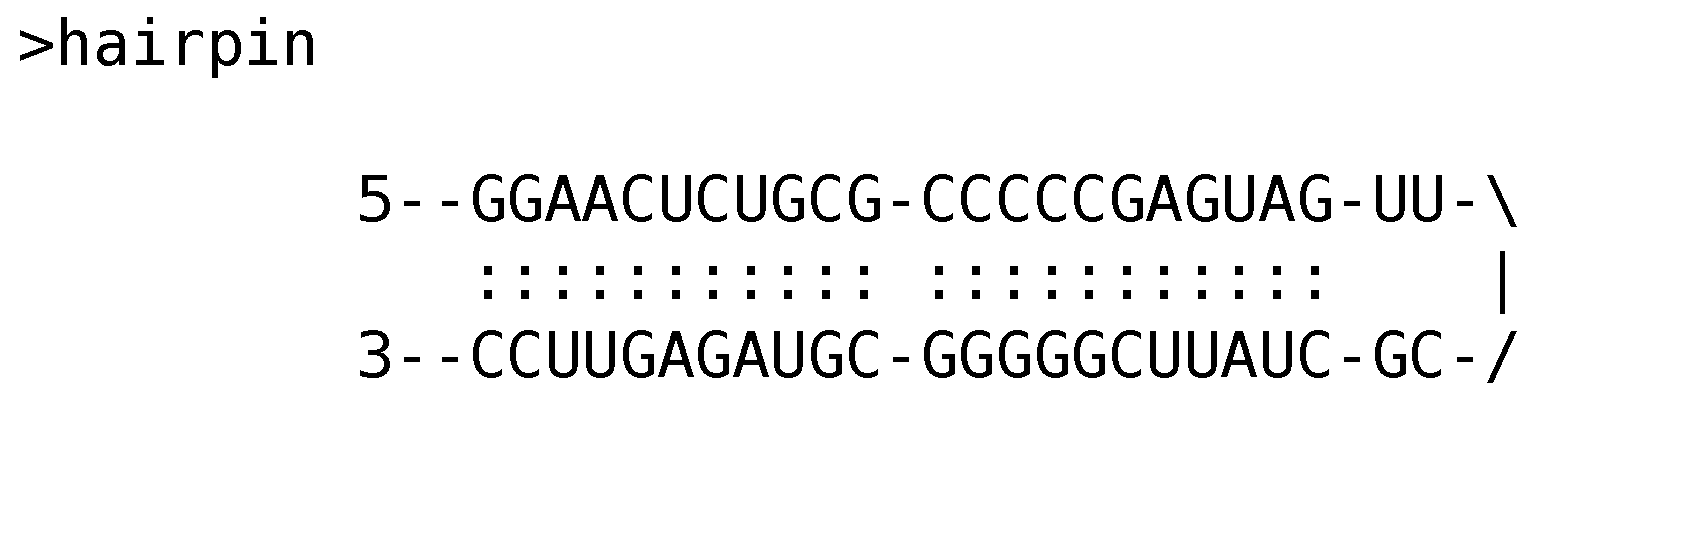
\includegraphics[align=c,width=\textwidth/3]{figures/oxrna_sims/hairpin.eps} \centering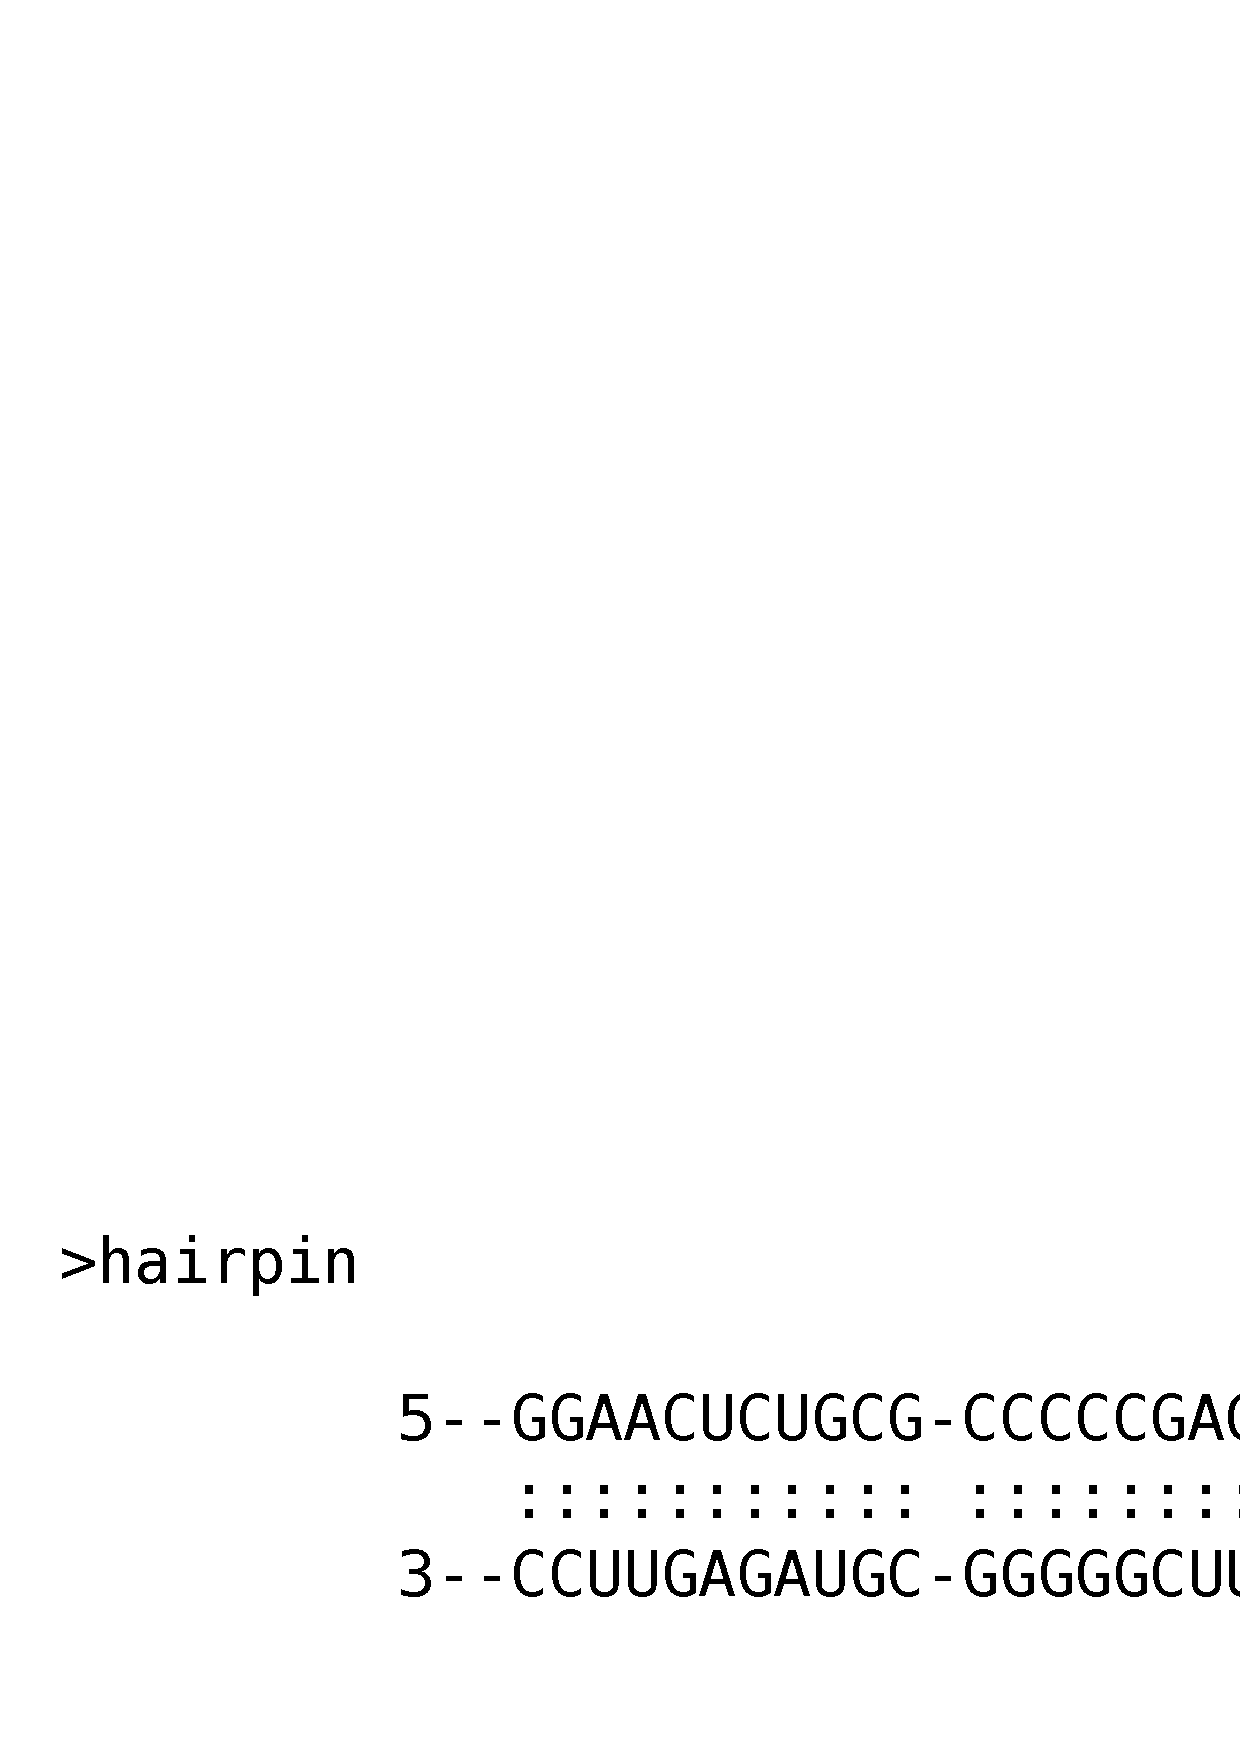
\includegraphics[align=c,width=\textwidth/3]{figures/oxrna_sims/hairpin.png} \centering\includegraphics[align=c,width=\textwidth/3]{figures/oxrna_sims/hairpin_last_conf.png}
}
\makebox[\textwidth][c]{b)  
  \centering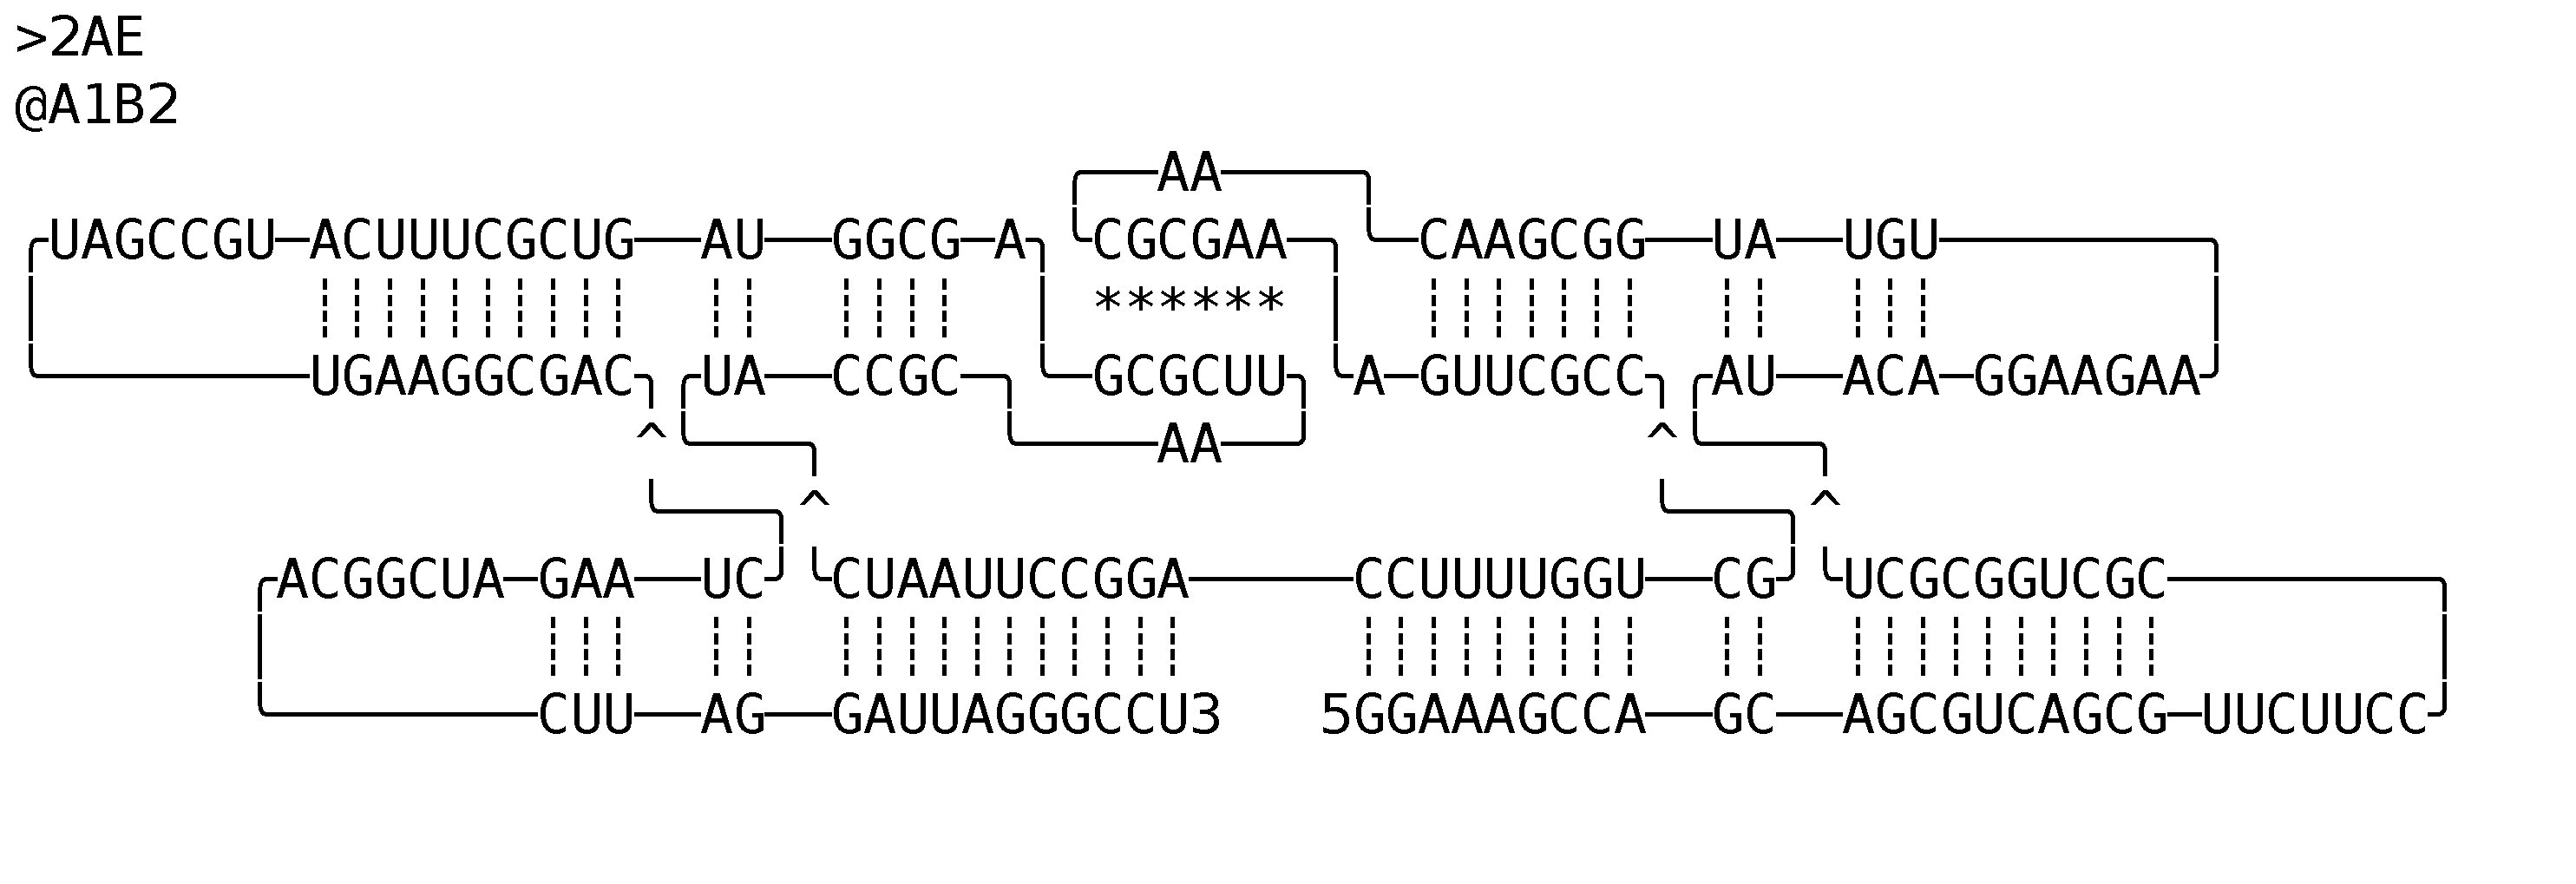
\includegraphics[align=c,width=\textwidth/3]{figures/oxrna_sims/2AE.eps} \centering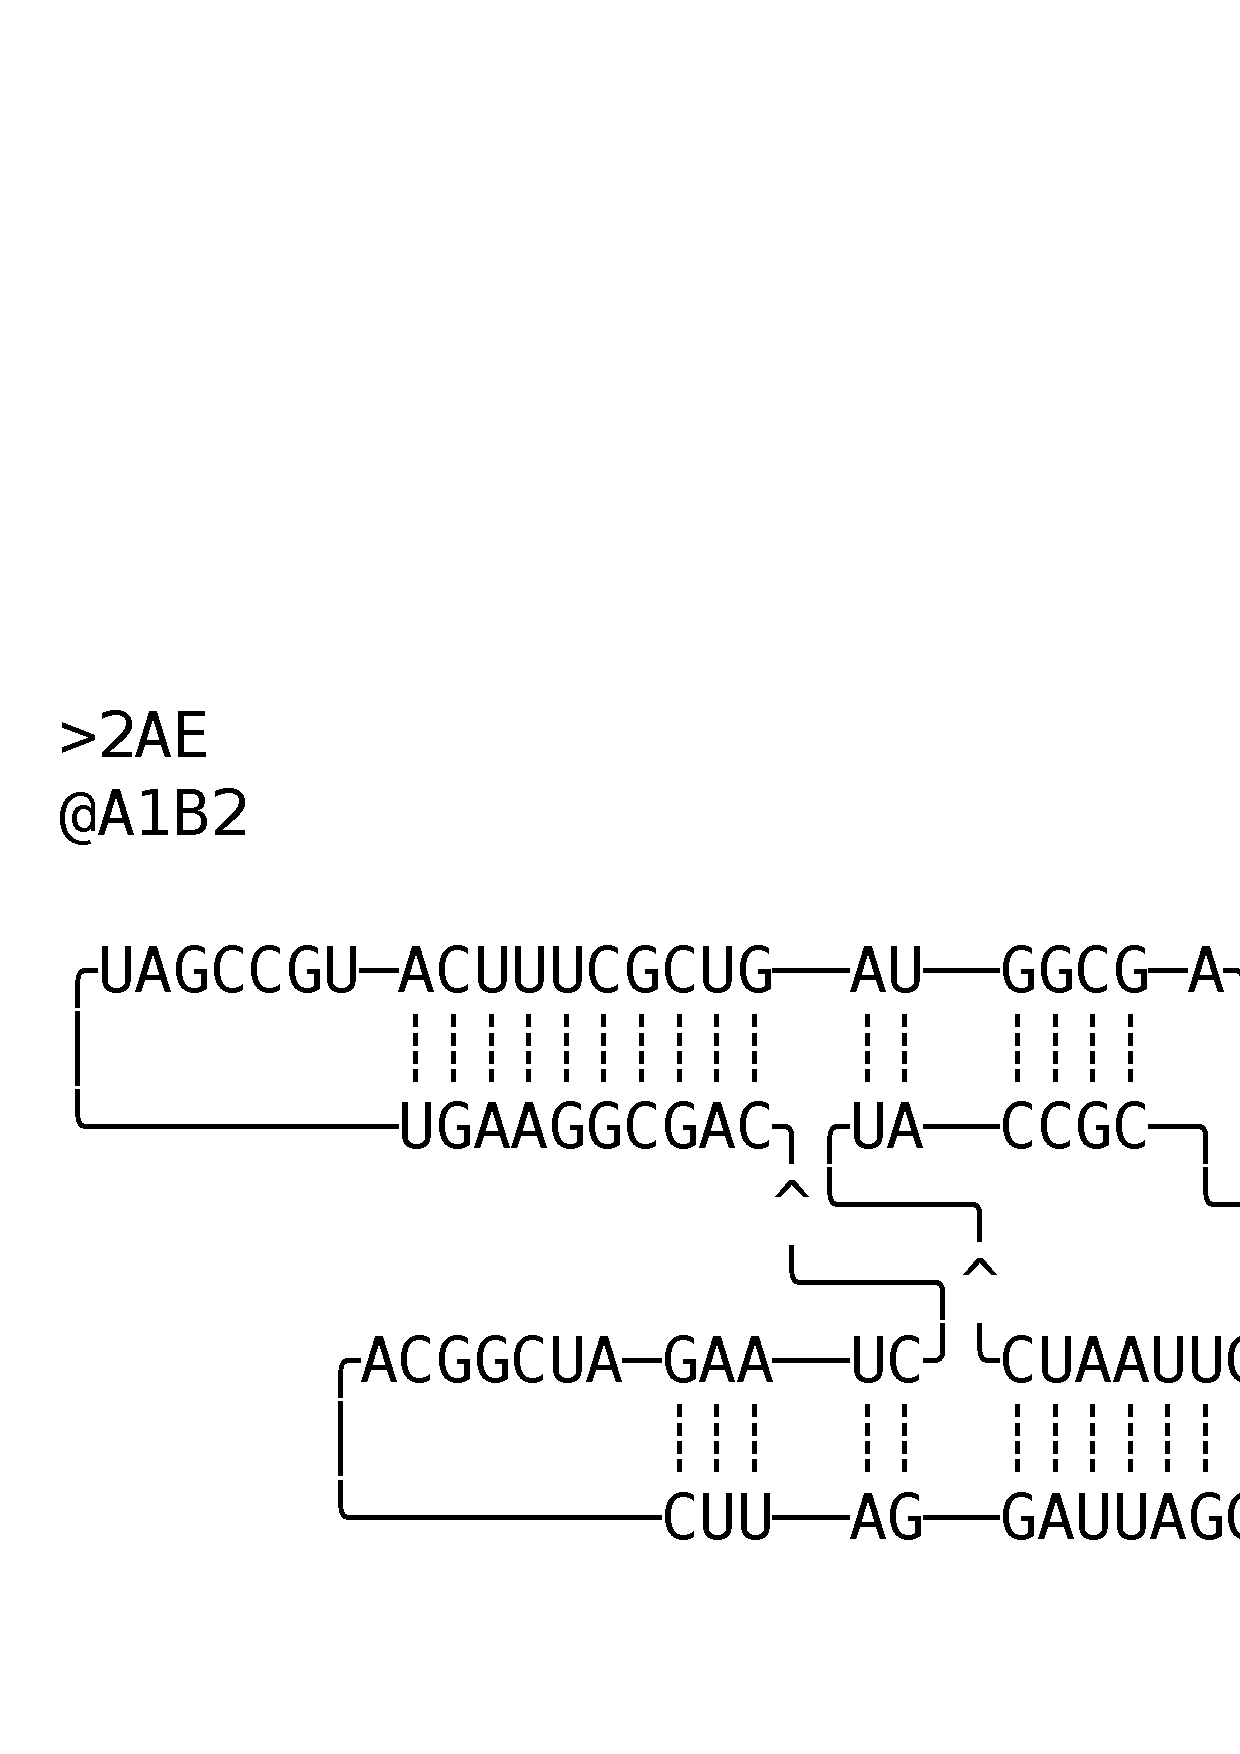
\includegraphics[align=c,width=\textwidth/3]{figures/oxrna_sims/2AE.png} \centering\includegraphics[align=c,width=\textwidth/3]{figures/oxrna_sims/2AE_last_conf.png}
}
\makebox[\textwidth][c]{c) 
  \centering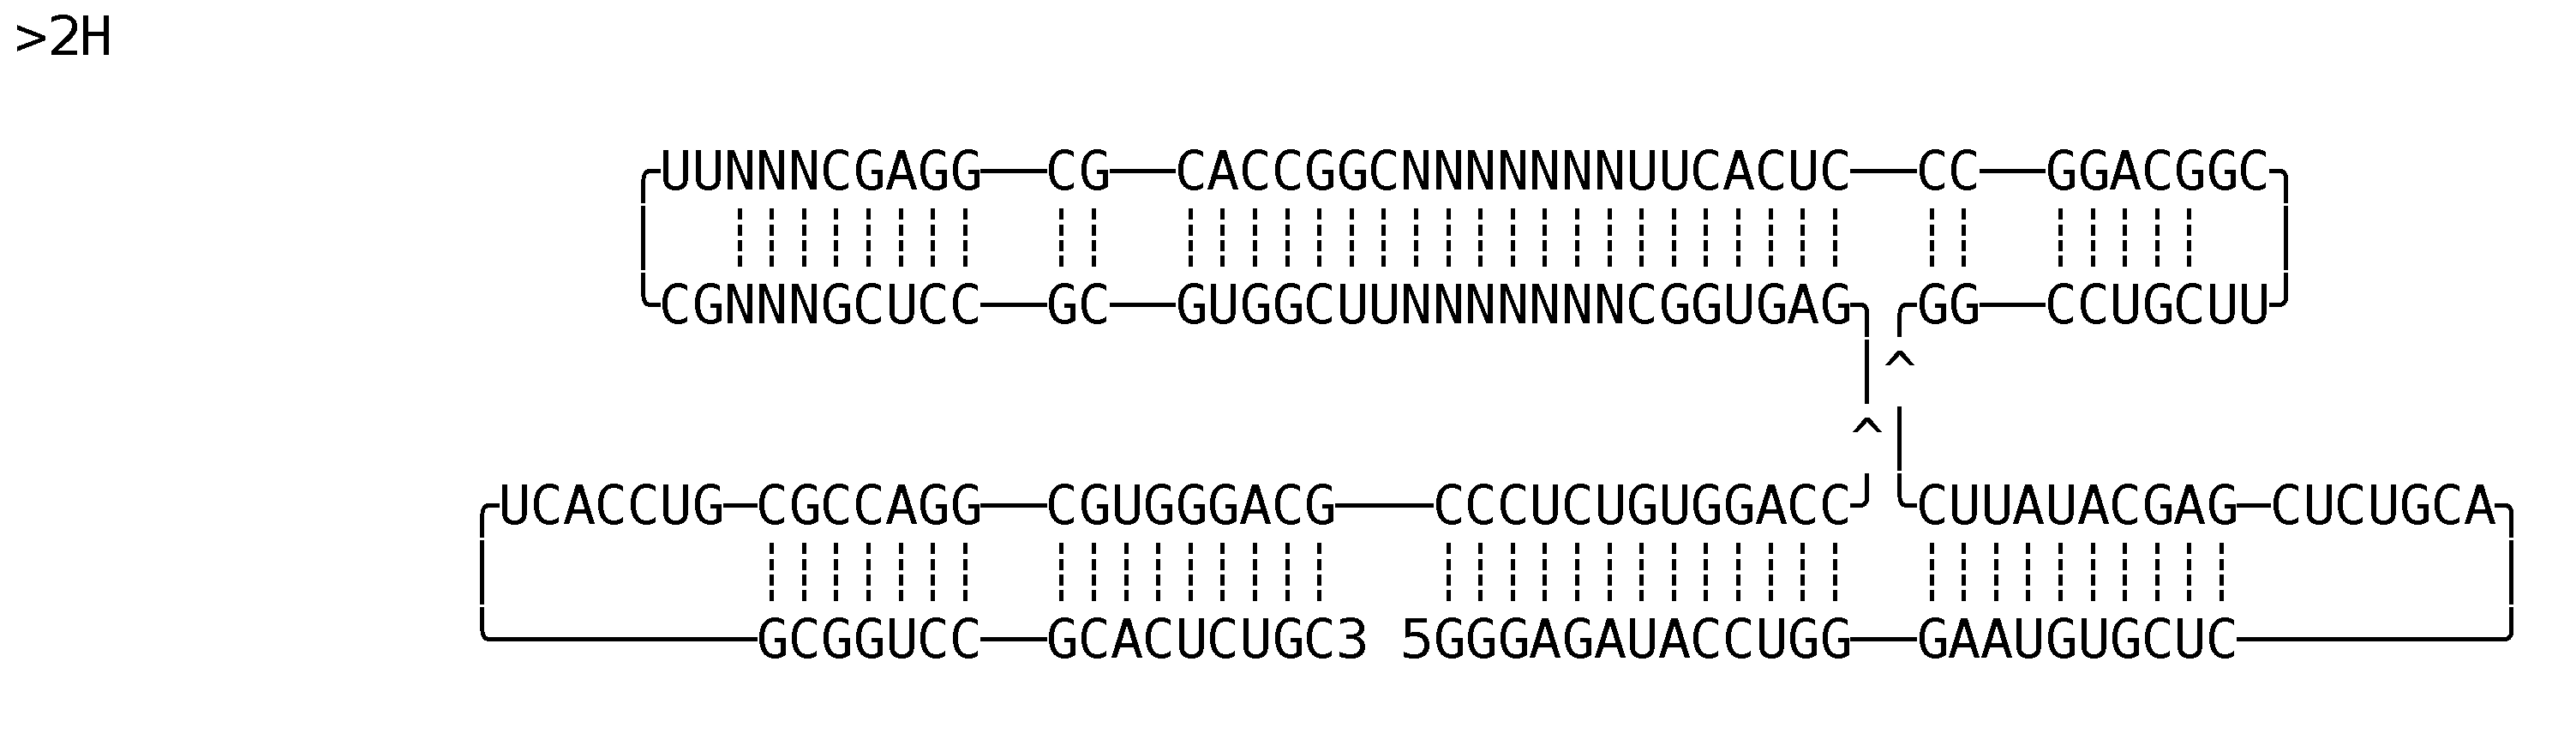
\includegraphics[align=c,width=\textwidth/3]{figures/oxrna_sims/2H.eps} \centering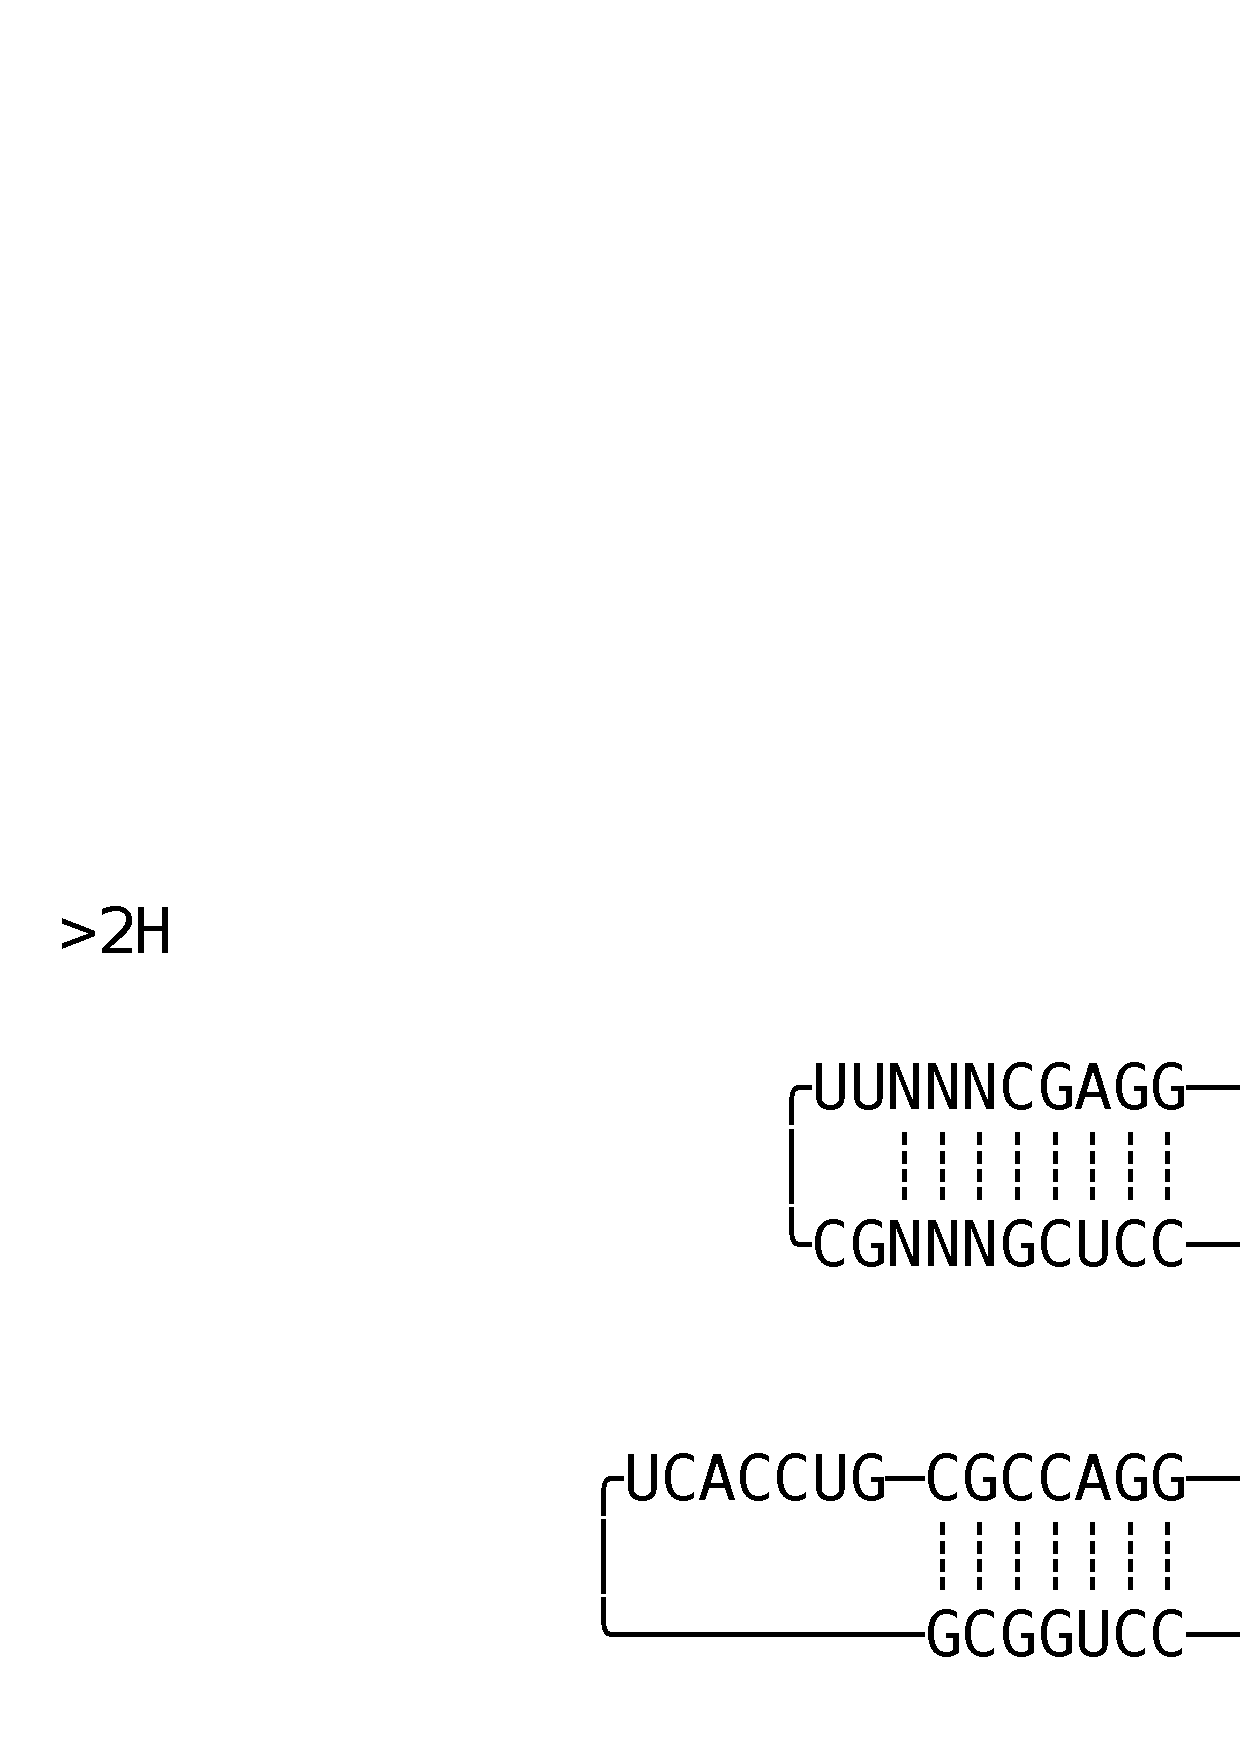
\includegraphics[align=c,width=\textwidth/3]{figures/oxrna_sims/2H.png}
  \centering\includegraphics[align=c,width=\textwidth/3]{figures/oxrna_sims/2H_last_conf.png}
}
\makebox[\textwidth][c]{d) 
  \centering\includegraphics[align=c,width=\textwidth/3]{figures/oxrna_sims/3H-Tri6.eps} \centering\includegraphics[align=c,width=\textwidth/3]{figures/oxrna_sims/3H-Tri6_pre.png}
  \centering\includegraphics[align=c,width=\textwidth/3]{figures/oxrna_sims/2H-Tri6_tri.png}
}
\makebox[\textwidth][c]{e)  
  \centering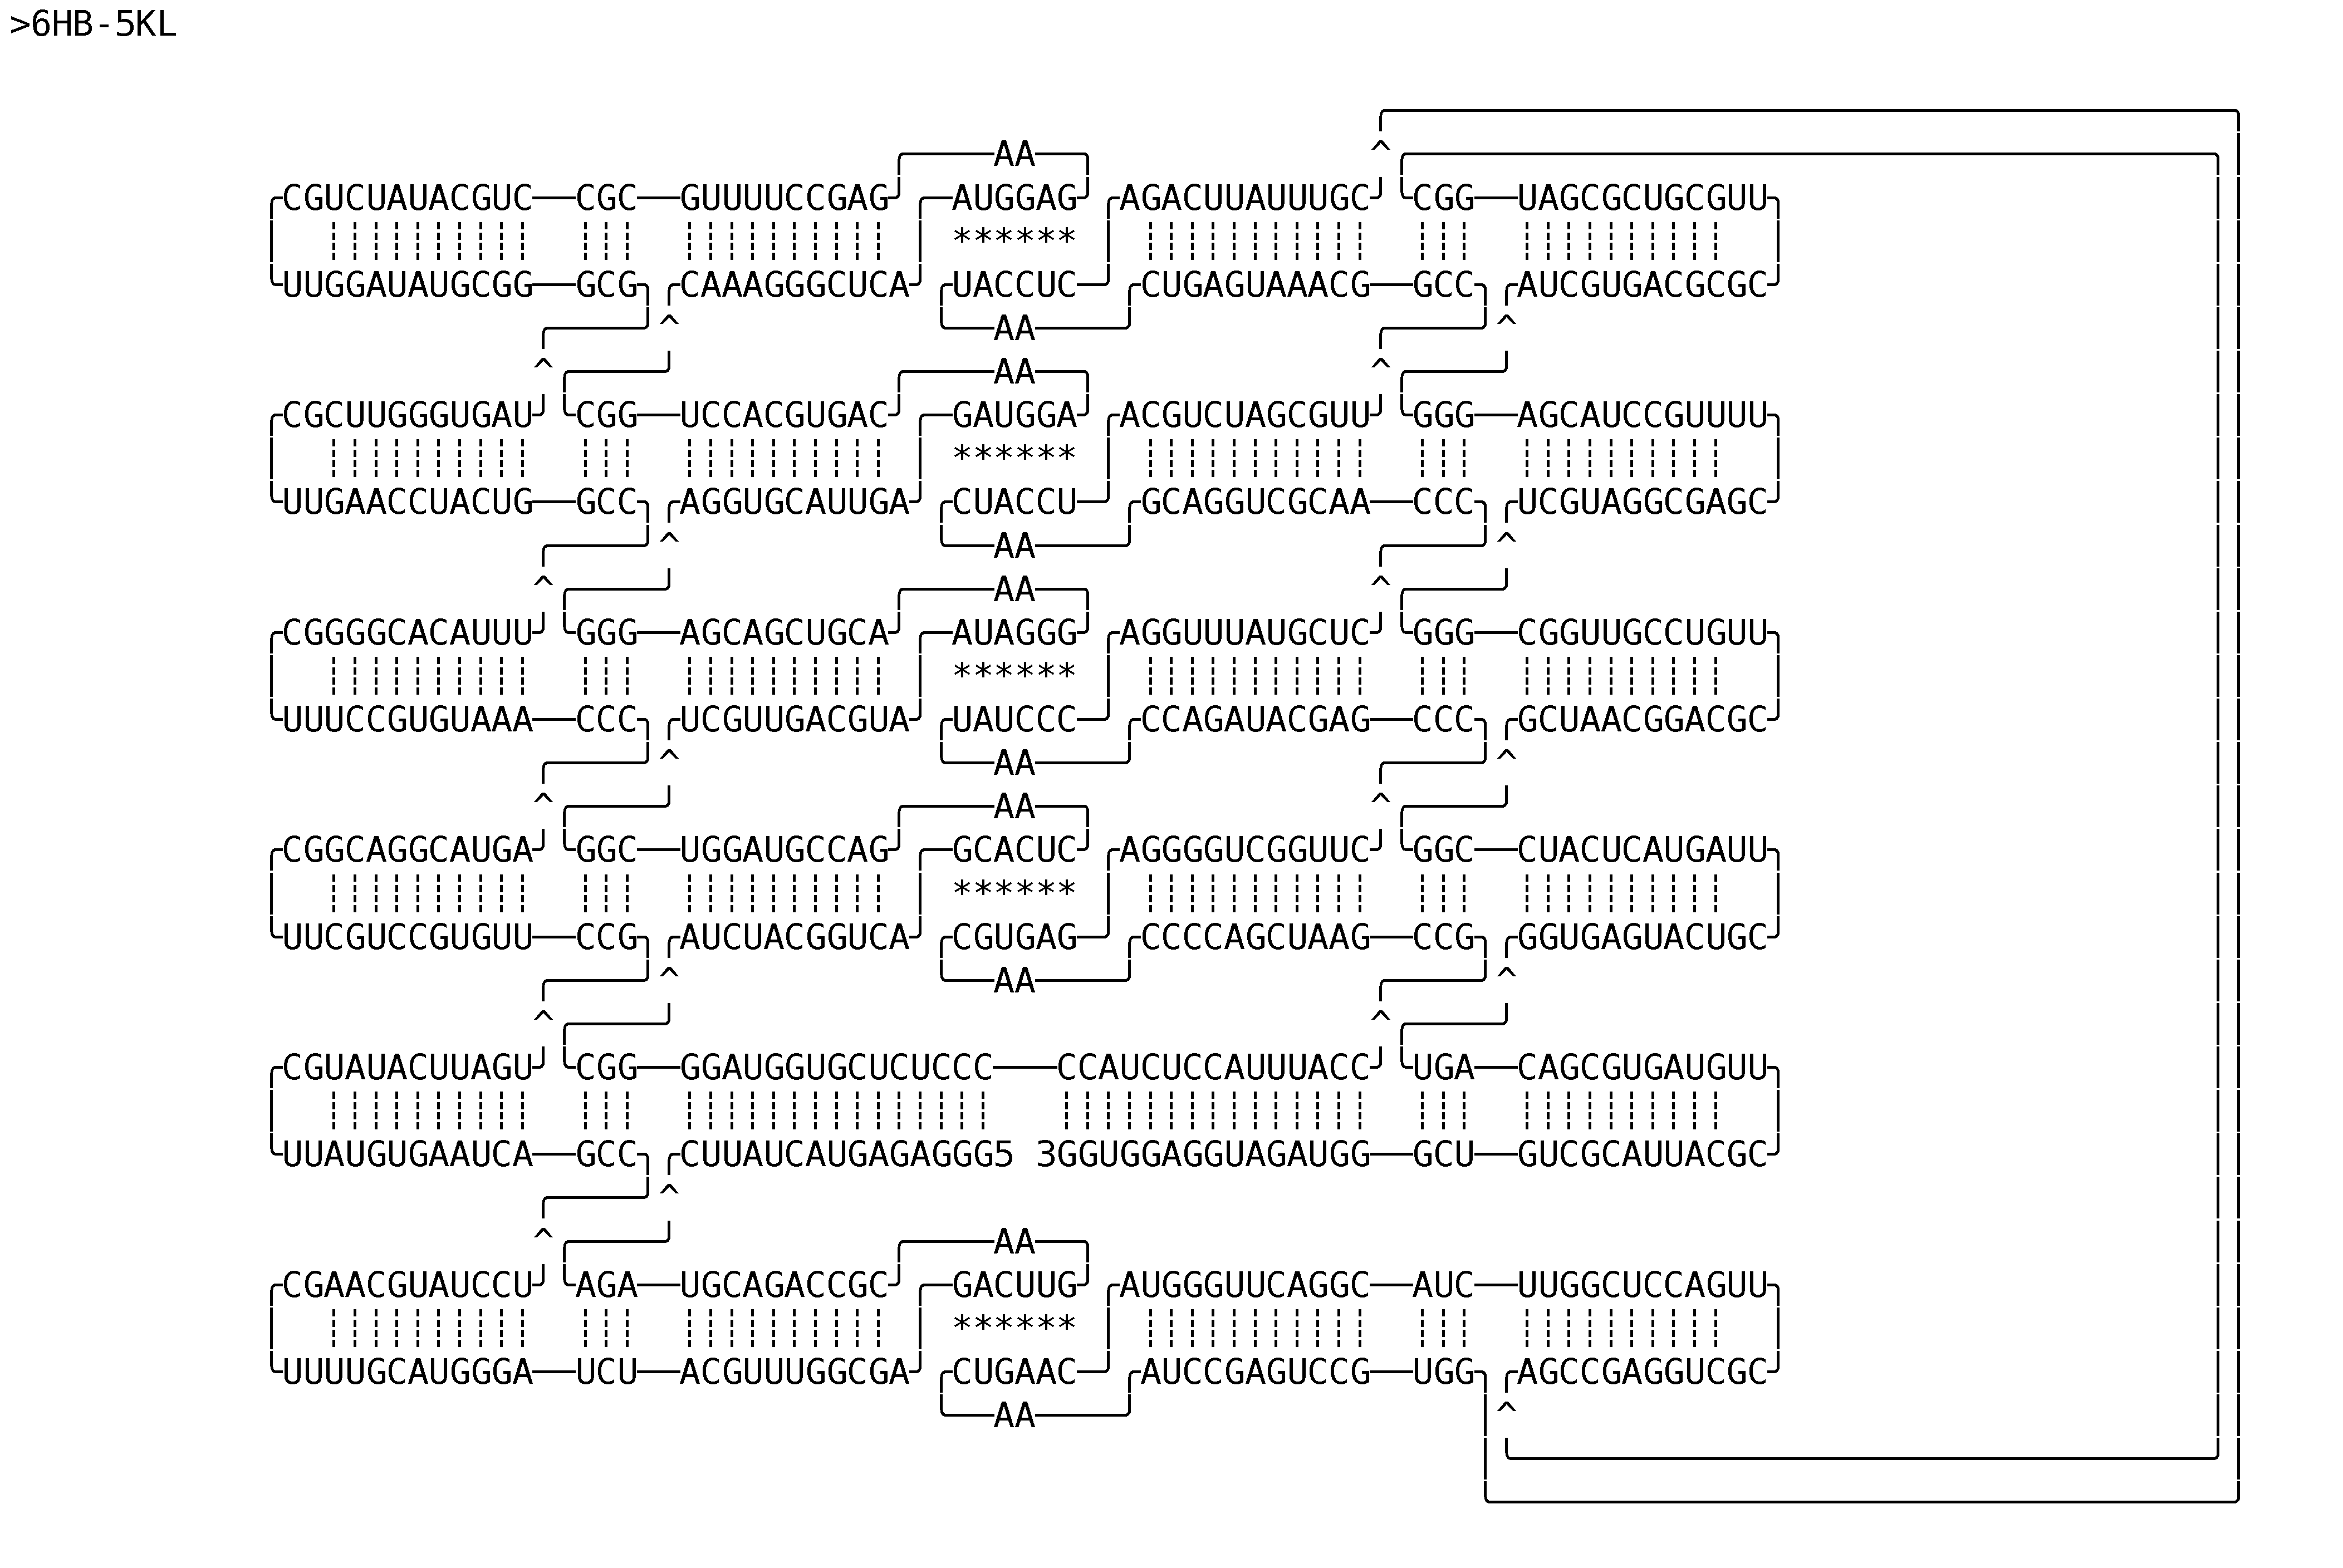
\includegraphics[align=c,width=\textwidth/3]{figures/oxrna_sims/6HB-5KL.eps} \centering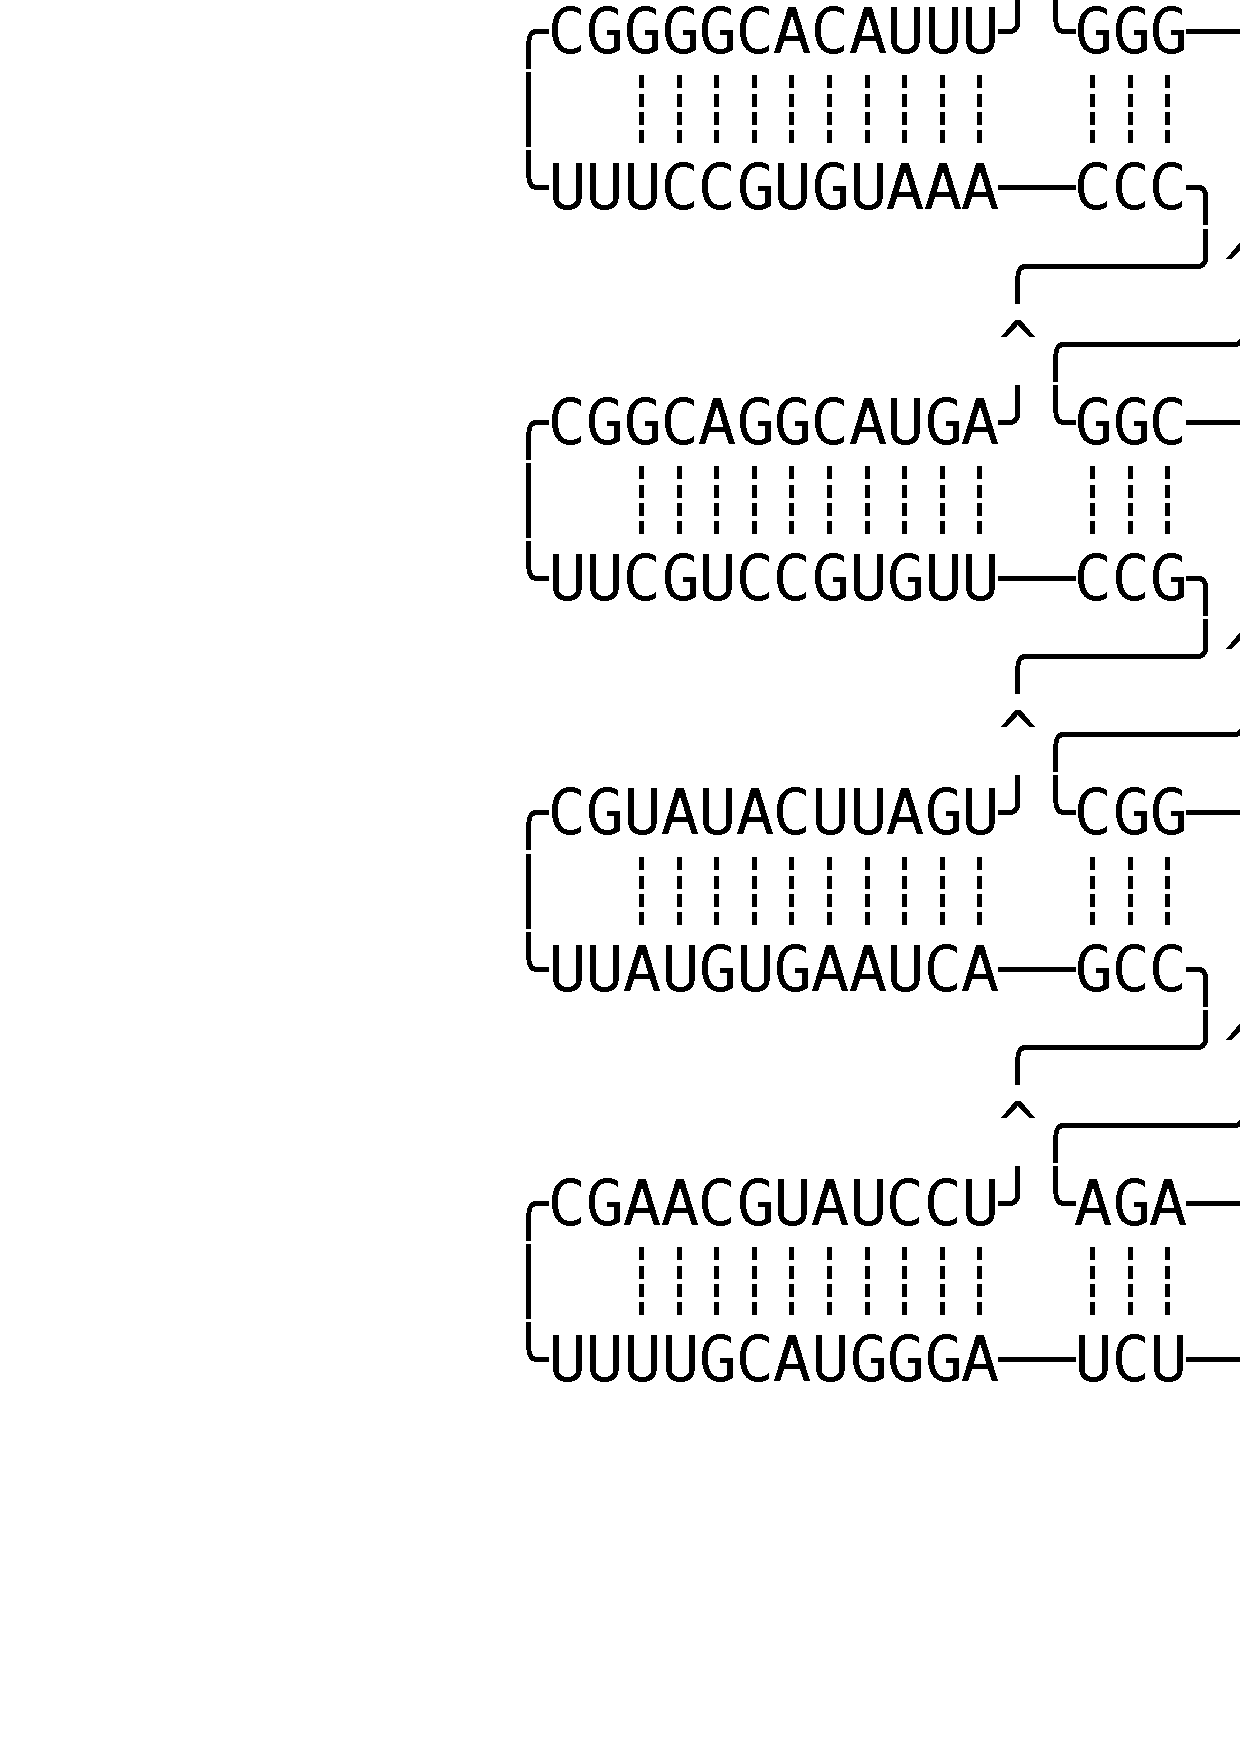
\includegraphics[align=c,width=\textwidth/3]{figures/oxrna_sims/6HB-5KL.png}
  \centering\includegraphics[align=c,width=\textwidth/3]{figures/oxrna_sims/6HB-5KL_last_conf.png}
}
\end{center}
\caption{Conversion and simulation of various RNA designs. Each row, from left to right, shows the ASCII blueprint design, the PDB model (visualised using ChimeraX), and a frame from the simulated structure (visualised using oxView). \textbf{a)} Is a simple hairpin loop. \textbf{b)} is a two-helix bundle tile used in \cite{geary2014single}. \textbf{c)} is two helices connected by a double crossover, analysing the flexibility of such a motif. \textbf{d)} is a possible design for a tensegrity triangle. \textbf{e)} is a siz-helix bundle.}
\label{fig:oxRNA_sims}\end{figure}



